\newpage

\section{Зависимость решений от начальных данных и параметров}

Пусть задано дифференциальное уравнение с параметром $\mu$:

$$\frac{dx}{dt} = f(t, x, \mu), \quad \mu = \begin{pmatrix}
  \mu_1 \\
  \vdots \\
  \mu_m
\end{pmatrix} \in \R^m$$

$$\frac{dx}{dt} = f(t, x), \quad f\in Lip_{x,\ loc}(G) \cap C(G) \quad \Rightarrow$$
$$\Rightarrow \quad \forall (\tau, \xi) \in G\ \ \exists!
\text{ решение задачи Коши с начальными данными } (\tau, \xi)$$

$$x(t, \tau, \xi, \mu) \text{ --- функция от $n+m+2$ переменных}$$


\begin{wrapfigure}{r}{0.5\textwidth}
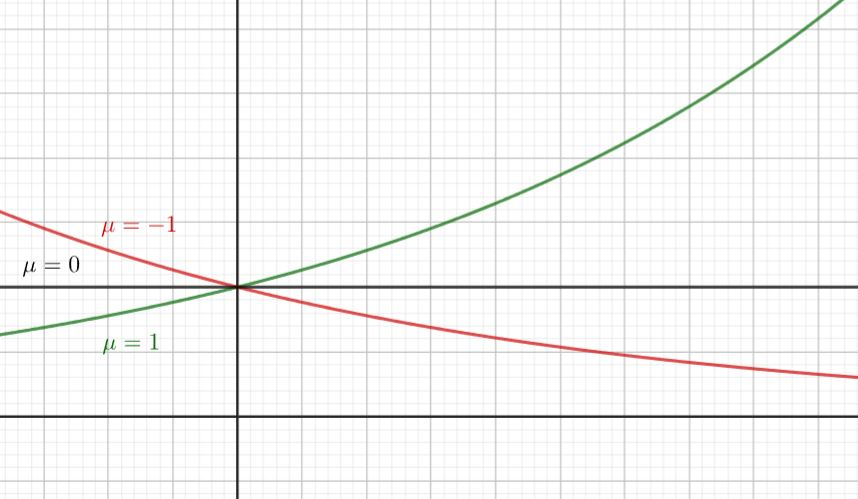
\includegraphics[width = 0.5\textwidth]{images/mu.JPG}
\end{wrapfigure}

Пример

$$\frac{dx}{dt} = \mu x, \quad x \in \R, \mu \in \R$$

$$x = Ce^{\mu x}$$

$$x(t, \tau, \xi, \mu) = \xi e^{\mu (t - \tau)}$$

\begin{itemize}
  \item $\mu = 0$ --- прямая $x = \xi$
  \item $\mu = 1$ --- экспонента
  \item $\mu = -1$ --- обратная экспонента
\end{itemize}


\vspace{10mm}
\subsection{Оценка разности двух решений}

Имеются две системы ДУ: $x,\, y \in \R^n,\, G\subset \R^{n+1}$,
$$
\begin{cases*}
  \dot{x} = f_1(t, x) \\
  \dot{y} = f_2(t, y)
\end{cases*}
$$

Предположим, что кроме условий существования и единственныости решения, выполняется еще

\begin{itemize}
  \item $f_1 \in Lip(G)$ с константой $L$
  \item $f_1$ ограничена ($|f_1| \leq M$)
  \item Ограниченность разности функций ($|f_1 - f_2|\leq m$)
\end{itemize}


\begin{theorem}
  Пусть решения $x(t, \tau_1, \xi_1)$ и $y(t, \tau_2, \xi_2)$ определены на $(a, b)$ и $\tau_1, \tau_2 \in (a, b)$.
  Тогда
  $$|x(t, \tau_1, \xi_1) - y(t, \tau_2, \xi_2)| \leq (|\xi_1 - \xi_2| + M|\tau_1 - \tau_2| + m(b - a))e^{L(b-a)}$$
\end{theorem}

Вспомним лемму Гронуолла, утверждающая, что при $\lambda,\, \mu \geq 0$ и $u(t) \in C$:

$$0 \leq u(t) \leq \lambda + \mu \left|\int_{t_0}^t u(s)\ ds \right|\quad \Rightarrow \quad u(t) \leq \lambda e^{\mu|t-t_0|}$$

\begin{proof}

  Решения $x$, $y$ удовлетворяют интегральным уравнениям
  $$
  \begin{gathered}
  x(t, \tau_1, \xi_1) = \xi_1 + \int_{\tau_1}^t f_1(s, x(s, \tau_1, \xi_1))\ ds \\
  y(t, \tau_2, \xi_2) = \xi_2 + \int_{\tau_2}^t f_2(s, y(s, \tau_2, \xi_2))\ ds \\
  \left|x(t, \tau_1, \xi_1) - y(t, \tau_2, \xi_2)\right| \leq |\xi_1 - \xi_2| + \left|\int_{\tau_1}^t f_1(s, x(s, \tau_1, \xi_1))\ ds - \int_{\tau_2}^t f_2(s, y(s, \tau_2, \xi_2))\ ds \right| = A \\
  \end{gathered}
  $$

  Не умаляя общности, $\tau_1 < \tau_2$
  
  $$
  \begin{gathered}
  A \leq |\xi_1 - \xi_2| + \left|\int_{\tau_1}^{\tau_2} f_1(s, x(s, \tau_1, \xi_1))\ ds\right| +  \left|\int_{\tau_2}^t f_1(s, x(s, \tau_1, \xi_1)) - f_2(s, y(s, \tau_2, \xi_2))\ ds \right| \leq \\
  \leq |\xi_1 - \xi_2| + M|\tau_1 - \tau_2| + \left| \int_{\tau_2}^t f_1(s, x(s, \tau_1, \xi_1)) - f_1(s, y(s, \tau_2, \xi_2))\ ds \right| + \\
  + \left| \int_{\tau_2}^t f_1(s, y(s, \tau_2, \xi_2)) - f_2(s, y(s, \tau_2, \xi_2))\ ds \right| \leq \\
  \leq |\xi_1 - \xi_2| + M|\tau_1 - \tau_2| + \left| \int_{\tau_2}^t L|x(s, \tau_1, \xi_1) - y(s, \tau_2, \xi_1)|\ ds\right| + m(b-a)
  \end{gathered}
  $$

  Итого
  $$\left|x(t, \tau_1, \xi_1) - y(t, \tau_2, \xi_2)\right| \leq \left(|\xi_1 - \xi_2| + M|\tau_1 - \tau_2| + m(b-a)\right) + L \left|\int_{\tau_2}^t x(s, \tau_1, \xi_1) - y(s, \tau_2, \xi_2) ds\right|$$

  Применяя лемму Гронуолла для $\lambda = \left(|\xi_1 - \xi_2| + M|\tau_1 - \tau_2| + m(b-a)\right)$, $\mu = L$ и $u(t) = \left|x(t, \tau_1, \xi_1) - y(t, \tau_2, \xi_2)\right|$, получаем утверждение задачи.

\end{proof}



\subsection{Теорема о непрерывной зависимости решения от начальных данных и параметров}

Дано дифференциальное уравнение:

$$\frac{dx}{dt} = f(t, x, \mu), \quad \mu \in \R^m = \mathfrak{M}$$

\begin{theorem}
  Пусть $f \in C(G \times \mathfrak{M}) \cap Lip_x(G \times \mathfrak{M})$ и пусть решение $x(t, \tau_0, \xi_0, \mu_0)$ определено на $(a, b)$.

  Тогда 

  $$\forall \epsilon>0 \, \exists \delta>0 \  \forall (\tau, \xi, \mu): \quad |\tau - \tau_0| < \delta,\ \ |\xi - \xi_0| < \delta,\ \  |\mu - \mu_0| < \delta$$

  решение $x(t, \tau, \xi, \mu)$ определено на $(a, b)$ и 

  $$|x(t, \tau, \xi, \mu) - x(t, \tau_0, \xi_0, \mu_0)| < \epsilon \quad \forall t \in (a, b)$$
\end{theorem}

\begin{wrapfigure}{r}{0.5\textwidth}
  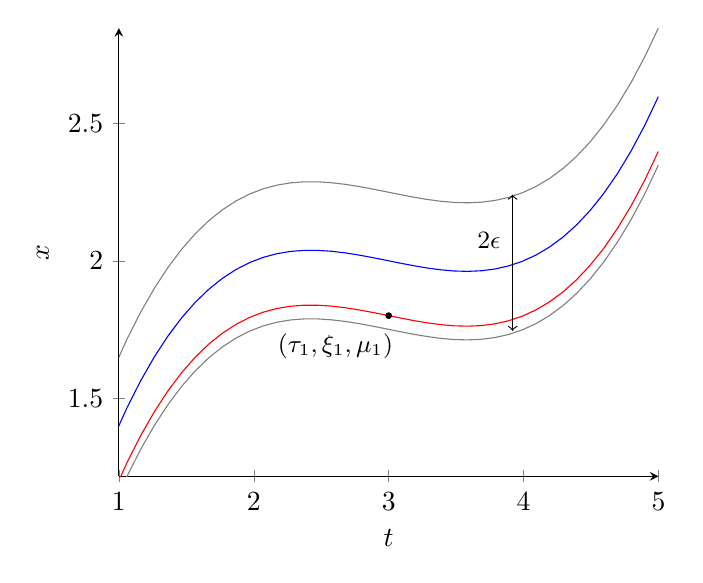
\begin{tikzpicture}
    \begin{axis}[
      axis lines = left,
      %title = Иллюстрация теоремы в двухмерном случае,
      xlabel = {$t$},
      ylabel = {$x$},
      xmin = 1,
      xmax = 5,
    ]
    \addplot[blue, samples = 100] {(x-2)*(x-3)*(x-4)/10 + 2};
    \addplot[gray, samples = 100] {(x-2)*(x-3)*(x-4)/10 + 1.75};
    \addplot[gray, samples = 100] {(x-2)*(x-3)*(x-4)/10 + 2.25};
    \addplot[
    samples = 20,
    mark size=1pt,
    only marks] coordinates {(3, 1.8)};
    \addplot[red, samples = 100] {(x-2)*(x-3)*(x-4)/10 + 1.8};

    \end{axis}

    \node at (2.75, 1.65) {\small $(\tau_1, \xi_1, \mu_1)$};
    \node at (4.7, 3) {\small $2\epsilon$};

    \draw[->] (5, 1.85) -- (5, 3.58);
    \draw[->] (5, 3.58) -- (5, 1.85);

    
  \end{tikzpicture}
\end{wrapfigure}

В данном курсе доказательство не приводится.